\subsection{Seq2SeqLSTMTrasformer}
La classe \texttt{Seq2SeqLSTMTrasformer} implementa un'architettura simile al modello Seq2SeqLSTM, ma inoltre aggiunge \(2\) blocchi Transformer sia nell'encoder che nel decoder.\\

\subsubsection{Encoder}
\begin{itemize}
    \item \textbf{Layer di embedding}
    \item \textbf{Due Blocchi Transformer} con:
        \begin{itemize}
            \item Dimensione latente pari a 300
            \item Dropout del 40\%
        \end{itemize}
    \item \textbf{Tre layer LSTM} con:
    \begin{itemize}
        \item Dimensione latente pari a 300
        \item Dropout del 40\%
        \item Recurrent dropout del 40\%
    \end{itemize}
\end{itemize}

\subsubsection{Decoder}
\begin{itemize}
    \item \textbf{Layer di embedding}
    \item \textbf{Due blocchi Transformer} con:
        \begin{itemize}
            \item Dimensione latente pari a 300
            \item Dropout del 40\%
            \item Recurrent dropout del 20\%
            \item Un MultiHeadAttention da \(8\) Head
            \item Un layer di Dropout del 10\%
            \item Un Add layer
            \item Un layer di Normalizzazione
            \item Tre layer di FeedForward con:
                \begin{itemize}
                    \item Un layer denso con attivazione ReLU e dimensione latente pari a \(512\)
                    \item Un layer denso con dimensione latente pari a \(300\)
                    \item Un layer di Dropout del 10\%
                    \item Un Add layer
                    \item Un layer di Normalizzazione
                \end{itemize}
        \end{itemize}
    \item \textbf{Layer LSTM} con:
        \begin{itemize}
            \item Stessa dimensione latente dell'encoder
            \item Dropout del 40\%
            \item Recurrent dropout del 40\%
        \end{itemize}
    \item \textbf{Layer di attention}
    \item \textbf{Layer denso di output}
\end{itemize}

Di seguito, possiamo vedere un diagramma dell'architettura del modello Seq2SeqLSTMTrasformer nella figura \ref{fig:seq2seqlstmtrasformer_model_architecture}.
\begin{figure}[H]
    \centering
    \includegraphics[width=0.55\textwidth]{media/Seq2SeqLSTMTransformer_image.png}
    \caption{Diagramma dell'architettura del modello Seq2SeqLSTMTrasformer}
    \label{fig:seq2seqlstmtrasformer_model_architecture}
\end{figure}

\training{Adam}{50}
\risultati{0.2015}{0.5034}{0.9576}{0.9269}

Possiamo verificare l'andamento della funzione di loss durante l'addestramento del modello nella figura \ref{fig:seq2seqlstmtrasformer_loss}.
\begin{figure}[H]
    \centering
    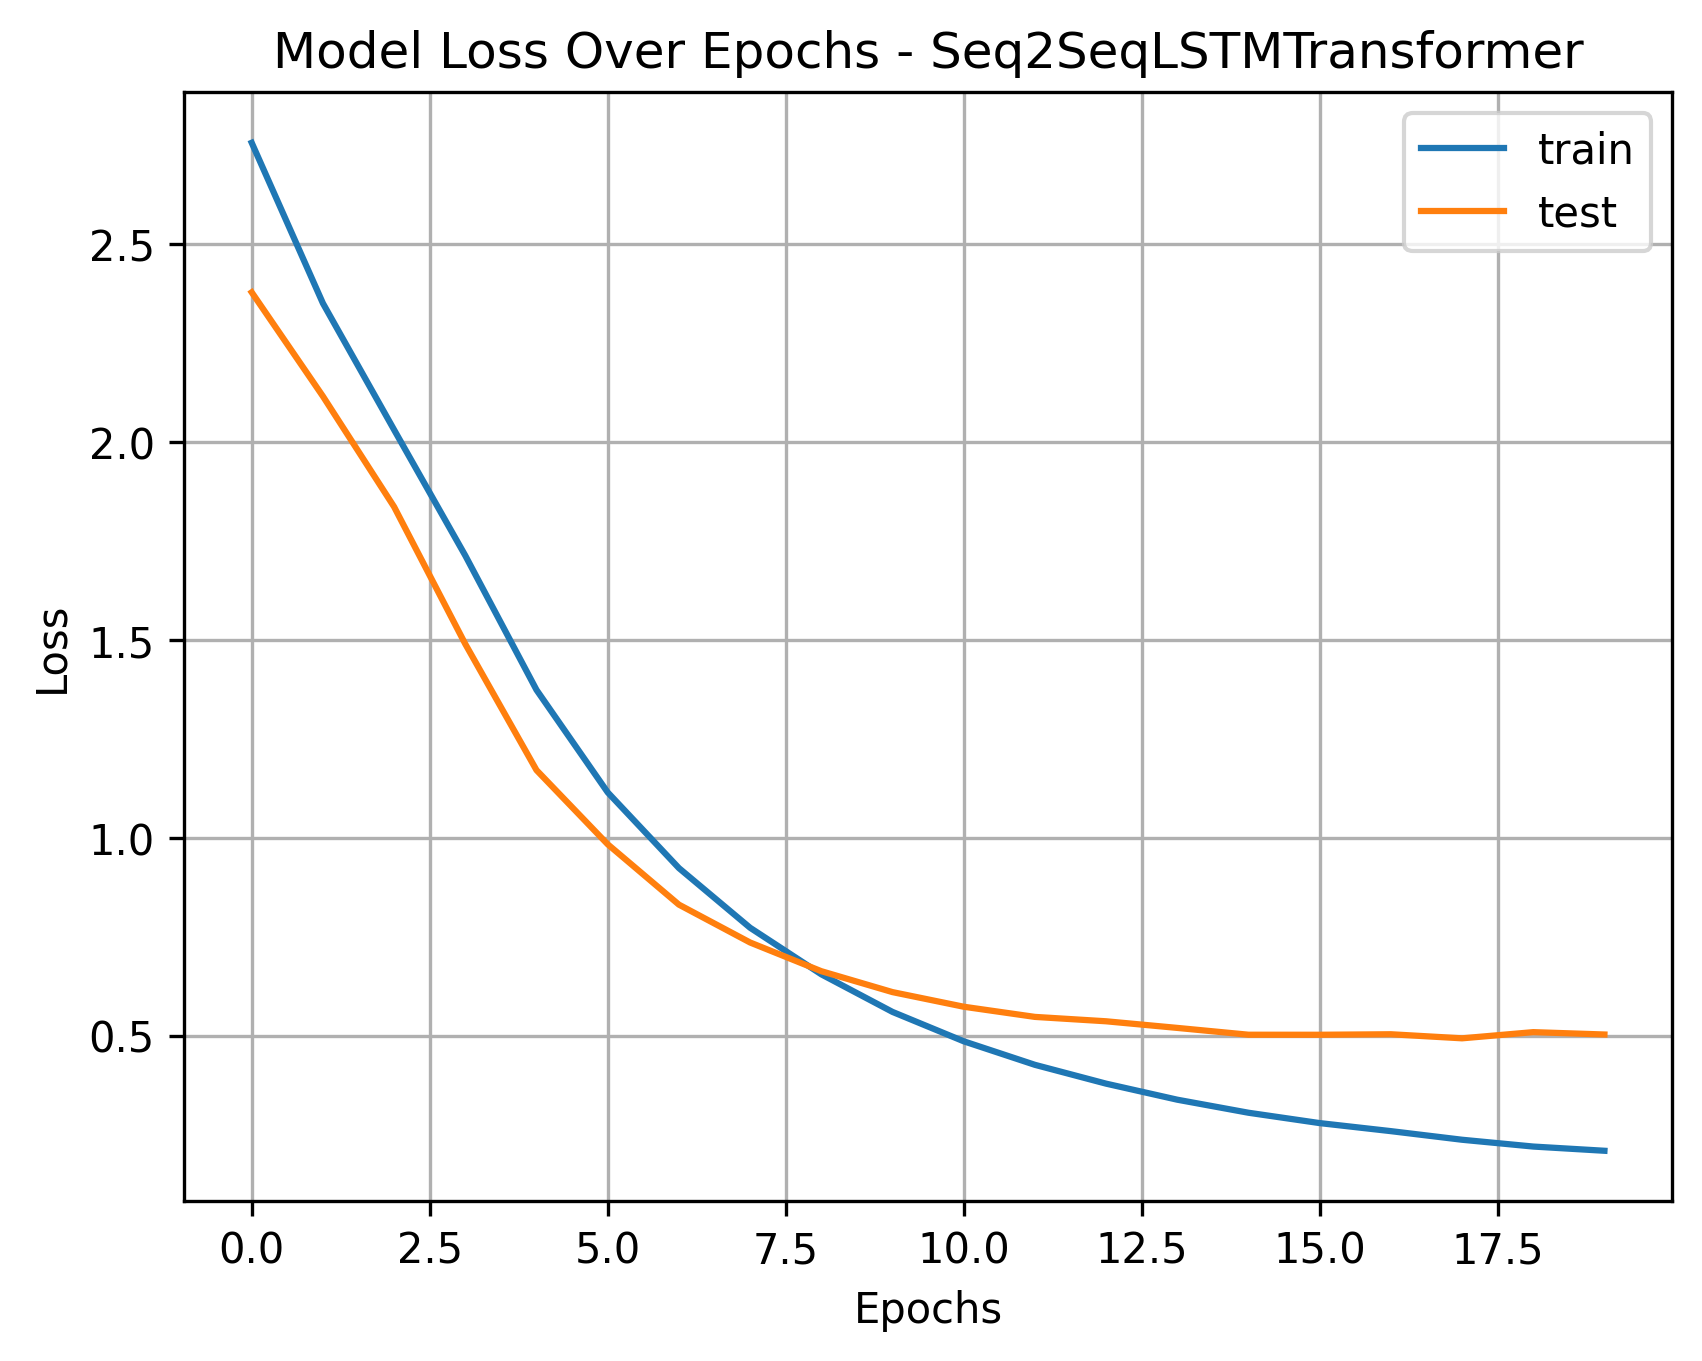
\includegraphics[width=0.65\textwidth]{media/Seq2SeqLSTMTransformer_originale_lossplot.png}
    \caption{Andamento della funzione di loss durante l'addestramento del modello Seq2SeqLSTMTrasformer}
    \label{fig:seq2seqlstmtrasformer_loss}
\end{figure}
